\begin{titlepage}
  \begin{tikzpicture}[remember picture, overlay]
    \node[anchor=center, inner sep=0pt] at (current page.center){
      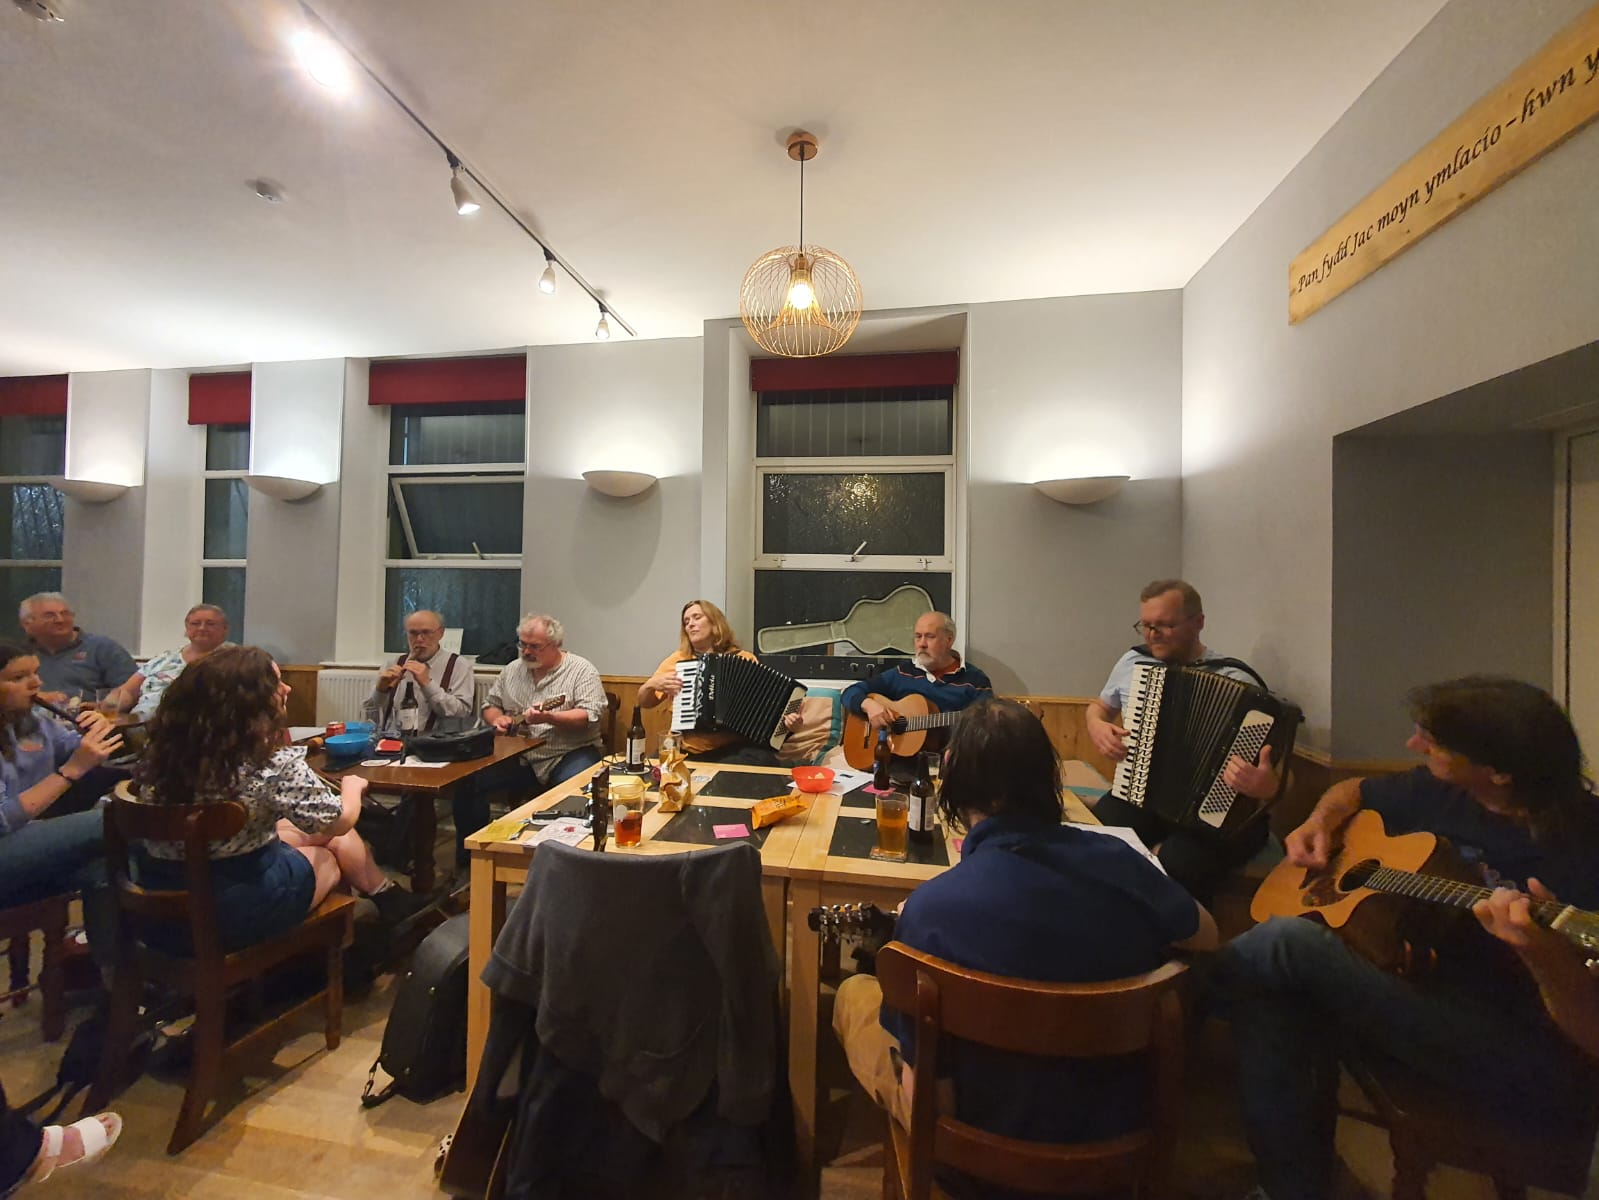
\includegraphics[
        width=\paperwidth,
        height=\paperheight,
        trim={{cover.trim|default("0 0 0 0")}}
      ]{../../assets/cover.jpg}
    };
    \node[
      fill=black,
      text=white,
      anchor=north east,
      xshift=20cm, yshift=13.5cm,
      opacity=0.7, text opacity=1
    ] at (current page.south west) {
      \fontsize{24}{48}\selectfont
      
    };

    \node[
      fill=white!20,
      anchor=south west,
      xshift={{title.xshift|default(1)}}cm,
      yshift={{title.yshift|default(3)}}cm,
      opacity=0.7, text opacity=1
    ] (title-node) at (current page.south west) {
      \fontsize{42}{48}\selectfont
        {{title.text|default("missing title.text property")}}
    };

    \node[
      fill=white!20,
      anchor={{subtitle.anchor|default("north west")}},
      xshift={{subtitle.xshift|default(2)}}cm,
      yshift={{subtitle.yshift|default(0.5)}}cm,
      opacity=0.7, text opacity=1
    ] (subtitle-node) at ({{subtitle.anchorTo|default("title-node.south west")}}) {
      \fontsize{17}{24}\selectfont
        {{subtitle.text|default("missing subtitle.text property")}}
    };

    \node[
      fill=black,
      text=white,
      anchor=south east,
      xshift=20cm, yshift=1cm,
      opacity=0.7, text opacity=1
    ] at (current page.south west) {
      \fontsize{17}{24}\selectfont
      
        {{titlenote.text|default("missing titlenote.text property")}}
      
        missing titlenote property
      
    };

  \end{tikzpicture}
\end{titlepage}